\documentclass[tikz,border=5pt]{standalone}
\usepackage[T1]{fontenc}
\usepackage{lmodern}
\usepackage{amsmath}
\usetikzlibrary{arrows.meta,calc}
\definecolor{ink}{HTML}{263747}
\definecolor{electrode}{HTML}{355F85}
\definecolor{ion}{HTML}{17877E}
\definecolor{pad}{HTML}{B67B24}
\definecolor{body}{HTML}{EDF1F4}
\definecolor{muted}{HTML}{65727C}
\begin{document}
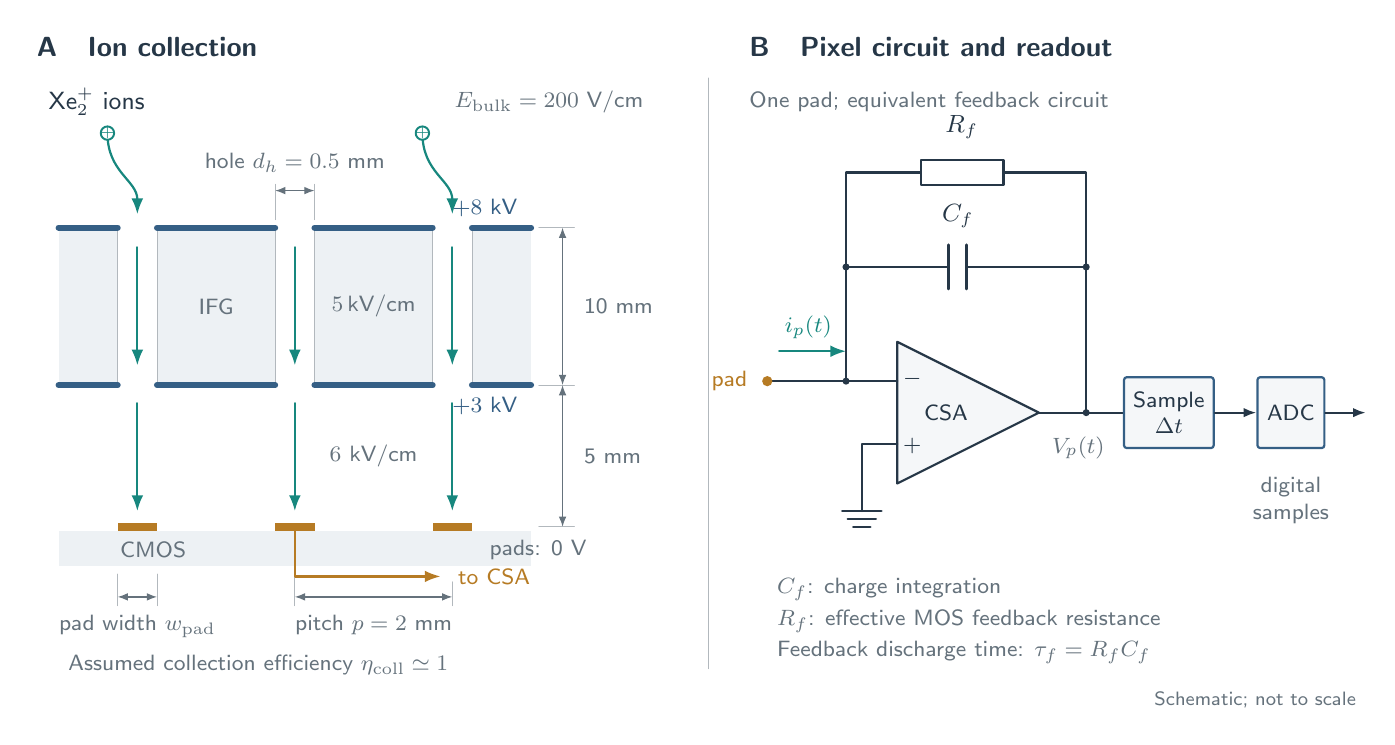
\begin{tikzpicture}[
    font=\sffamily\small, text=ink,
    line cap=round, line join=round,
    wire/.style={draw=ink,line width=.8pt},
    flow/.style={draw=ion,line width=.8pt,-{Latex[length=2mm]}},
    dim/.style={draw=muted,line width=.45pt,{Latex[length=1.3mm]}-{Latex[length=1.3mm]}},
    guide/.style={draw=muted!50,line width=.35pt},
    block/.style={draw=electrode,line width=.8pt,fill=electrode!5,rounded corners=1pt,align=center},
    labeltext/.style={font=\sffamily\footnotesize,text=muted}
]

% Geometry is a section through three round holes. Dimensions are nominal;
% vertical distances are compressed for legibility. This is not a field solve.
\node[anchor=west,font=\sffamily\bfseries] at (0,7.15) {A\quad Ion collection};
\node[anchor=west,font=\sffamily\bfseries] at (9.05,7.15) {B\quad Pixel circuit and readout};
\draw[guide] (8.65,-.75) -- (8.65,6.75);

\node[anchor=west] at (.15,6.45) {Xe$_2^+$ ions};
\node[anchor=east,labeltext] at (7.95,6.45) {$E_{\mathrm{bulk}}=200$ V/cm};

% IFG body and open channels; no electrical boundary condition is assigned
% to the vertical walls in this schematic.
\fill[body] (.4,2.85) rectangle (6.4,4.85);
\foreach \xc in {1.4,3.4,5.4} {
    \fill[white] ({\xc-.25},2.85) rectangle ({\xc+.25},4.85);
    \draw[guide] ({\xc-.25},2.85) -- ({\xc-.25},4.85);
    \draw[guide] ({\xc+.25},2.85) -- ({\xc+.25},4.85);
}
\foreach \ya in {2.85,4.85} {
    \foreach \xa/\xb in {.4/1.15,1.65/3.15,3.65/5.15,5.65/6.4} {
        \draw[electrode,line width=2.2pt] (\xa,\ya) -- (\xb,\ya);
    }
}
\node[anchor=east,text=electrode,font=\sffamily\footnotesize] at (6.35,5.1) {$+8$ kV};
\node[anchor=east,text=electrode,font=\sffamily\footnotesize] at (6.35,2.58) {$+3$ kV};
\node[align=center,labeltext] at (2.4,3.85) {IFG};
\node[align=center,labeltext] at (4.4,3.85) {$5$\,kV/cm};

% Illustrative approach paths, not numerically calculated field lines.
\foreach \xc in {1.4,5.4} {
    \draw[flow] ({\xc-.38},6.05) .. controls ({\xc-.38},5.55) and (\xc,5.45) .. (\xc,5.02);
    \draw[ion,fill=white,line width=.7pt] ({\xc-.38},6.05) circle (.085);
    \node[font=\sffamily\tiny,text=ion] at ({\xc-.38},6.05) {$+$};
}
\foreach \xc in {1.4,3.4,5.4} {
    \draw[flow] (\xc,4.6) -- (\xc,3.1);
    \draw[flow] (\xc,2.62) -- (\xc,1.25);
}

% Hole diameter and vertical dimensions.
\draw[guide] (3.15,4.95) -- (3.15,5.4);
\draw[guide] (3.65,4.95) -- (3.65,5.4);
\draw[dim] (3.15,5.32) -- (3.65,5.32);
\node[labeltext,anchor=south] at (3.4,5.43) {hole $d_h=0.5$ mm};
\draw[guide] (6.5,4.85) -- (6.95,4.85);
\draw[guide] (6.5,2.85) -- (6.95,2.85);
\draw[dim] (6.8,2.85) -- (6.8,4.85);
\node[anchor=west,labeltext] at (6.95,3.85) {10 mm};
\draw[guide] (6.5,1.05) -- (6.95,1.05);
\draw[dim] (6.8,1.05) -- (6.8,2.85);
\node[anchor=west,labeltext] at (6.95,1.95) {5 mm};
\node[labeltext] at (4.4,1.95) {$6$ kV/cm};

% Isolated pads on a schematic CMOS surface: the spaces between pads are
% deliberately not drawn as a grounded metal plane.
\fill[body] (.4,.55) rectangle (6.4,1.0);
\node[labeltext] at (1.6,.76) {CMOS};
\foreach \xc in {1.4,3.4,5.4} {
    \fill[pad] ({\xc-.25},1.0) rectangle ({\xc+.25},1.1);
}
\node[anchor=west,labeltext] at (5.75,.75) {pads: 0 V};
\draw[guide] (3.4,.45) -- (3.4,.05);
\draw[guide] (5.4,.35) -- (5.4,.05);
\draw[dim] (3.4,.16) -- (5.4,.16);
\node[anchor=north,labeltext] at (4.4,.05) {pitch $p=2$ mm};
\draw[guide] (1.15,.45) -- (1.15,.05);
\draw[guide] (1.65,.45) -- (1.65,.05);
\draw[dim] (1.15,.16) -- (1.65,.16);
\node[anchor=north,labeltext] at (1.4,.05) {pad width $w_{\mathrm{pad}}$};
\draw[pad,line width=.8pt,-{Latex[length=2mm]}] (3.4,1.0) -- (3.4,.42) -- (5.25,.42);
\node[anchor=west,labeltext,text=pad] at (5.35,.42) {to CSA};
\node[anchor=west,labeltext] at (.4,-.7) {Assumed collection efficiency $\eta_{\mathrm{coll}}\simeq1$};

% Equivalent CSA: the resistor represents the MOS feedback discharge path.
\begin{scope}[shift={(9.05,0)}]
    \node[anchor=west,labeltext] at (0,6.45) {One pad; equivalent feedback circuit};
    \draw[wire,fill=electrode!5] (2,1.6) -- (2,3.4) -- (3.8,2.5) -- cycle;
    \node[font=\sffamily\footnotesize] at (2.62,2.5) {CSA};
    \node[font=\sffamily\footnotesize] at (2.19,2.93) {$-$};
    \node[font=\sffamily\footnotesize] at (2.19,2.08) {$+$};
    \draw[wire] (.35,2.9) -- (2,2.9);
    \fill[pad] (.35,2.9) circle (.065);
    \node[anchor=east,text=pad,font=\sffamily\footnotesize] at (.22,2.9) {pad};
    \draw[flow] (.5,3.28) -- (1.35,3.28);
    \node[anchor=south,text=ion,font=\sffamily\footnotesize] at (.87,3.32) {$i_p(t)$};
    \draw[wire] (2,2.1) -- (1.55,2.1) -- (1.55,1.25);
    \draw[wire] (1.3,1.25) -- (1.8,1.25);
    \draw[wire] (1.37,1.15) -- (1.73,1.15);
    \draw[wire] (1.44,1.05) -- (1.66,1.05);

    \draw[wire] (3.8,2.5) -- (4.95,2.5);
    \node[anchor=north,labeltext] at (4.3,2.32) {$V_p(t)$};
    \draw[wire] (1.35,2.9) -- (1.35,4.35) -- (2.65,4.35);
    \draw[wire,line width=1.05pt] (2.65,4.07) -- (2.65,4.63);
    \draw[wire,line width=1.05pt] (2.88,4.07) -- (2.88,4.63);
    \draw[wire] (2.88,4.35) -- (4.4,4.35) -- (4.4,2.5);
    \node[anchor=south] at (2.77,4.73) {$C_f$};
    \draw[wire] (1.35,4.35) -- (1.35,5.55) -- (2.3,5.55);
    \draw[wire,fill=white] (2.3,5.39) rectangle (3.35,5.71);
    \draw[wire] (3.35,5.55) -- (4.4,5.55) -- (4.4,4.35);
    \node[anchor=south] at (2.82,5.85) {$R_f$};
    \foreach \x/\y in {1.35/2.9,1.35/4.35,4.4/4.35,4.4/2.5} {
        \fill[ink] (\x,\y) circle (.045);
    }

    \node[block,minimum width=1.0cm,minimum height=.9cm,font=\sffamily\footnotesize] (sampling) at (5.45,2.5) {Sample\\$\Delta t$};
    \node[block,minimum width=.85cm,minimum height=.9cm,font=\sffamily\footnotesize] (adc) at (7.0,2.5) {ADC};
    \draw[wire,-{Latex[length=1.6mm]}] (sampling.east) -- (adc.west);
    \draw[wire,-{Latex[length=1.6mm]}] (adc.east) -- (7.95,2.5);
    \node[anchor=north,align=center,labeltext] at (7.0,1.8) {digital\\samples};

    \node[anchor=west,labeltext] at (.35,.25) {$C_f$: charge integration};
    \node[anchor=west,labeltext] at (.35,-.15) {$R_f$: effective MOS feedback resistance};
    \node[anchor=west,labeltext] at (.35,-.55) {Feedback discharge time: $\tau_f=R_fC_f$};
\end{scope}
\node[anchor=east,font=\sffamily\scriptsize,text=muted] at (17,-1.15) {Schematic; not to scale};
\end{tikzpicture}
\end{document}
